\begin{figure}[htbp]
    \centering
    \begin{minipage}{0.2\textwidth}
        \centering
        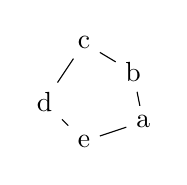
\begin{tikzpicture}[scale = 0.5]
            % Nodes with manual coordinates
            \node (a) at (1,-5.5) {a};
            \node (c) at (-0.5,-3.5) {c};
            \node (b) at (0.75, -4.25) {b};
            \node (d) at (-1.5,-5) {d};
            \node (e) at (-0.5,-6) {e};
            
            % Edges
            \draw (b) -- (a);
            \draw (c) -- (b);
            \draw (c) -- (d);
            \draw (a) -- (e);
            \draw (e) -- (d);
        \end{tikzpicture}
        \caption{$G$.}
    \end{minipage}
    \begin{minipage}{0.2\textwidth}
        \centering
        \tikz [tree layout, grow=-90,
               sibling distance=11mm, level distance=10mm, scale = 0.5]
          \graph {
            ""[as=$c$] ->
            ""[as=$a$] -> { ""[as=$b$], ""[as=$d$] -> {""[as=$e$]}}
          };
        \caption{$D^*$.}
    \end{minipage}
    \pause
    \begin{minipage}{0.55\textwidth}
        \centering
        \begin{tikzpicture}[scale = 0.5]
            \draw [decorate, 
       decoration = {calligraphic brace, amplitude = 5pt, mirror}, 
       line width = 1.5pt] 
      (-1.75,-3.2) -- (-1.75,-7.8);
            % Nodes with manual coordinates
            \node (a) at (1,-5.5) {a};
            \node (c) at (-0.5,-3.5) {c};
            \node (b) at (0.75, -4.25) {b};
            \node (d) at (-1.5,-5) {d};
            \node (e) at (-0.5,-6) {e};

            
            % Edges
            \draw (b) -- (a);
            \draw (c) -- (b);
            \draw (c) -- (d);
            \draw (a) -- (e);
            \draw (e) -- (d);
            
            \node at (1.3, -6.2) {,};

            \node (a2) at (4.5,-5.5) {a};
            \node (b2) at (4.25, -4.25) {b};
            \node (d2) at (2,-5) {d};
            \node (e2) at (3,-6) {e};
            
            % Edges
            \draw (b2) -- (a2);
            \draw (a2) -- (e2);
            \draw (e2) -- (d2);

            \node at (4.75, -6.2) {,};

            \node (b3) at (1.75, -7.4) {b};

            
            \node at (-0.2, -7.7) {,};

            \node (d3) at (-1.5,-6.5) {d};
            \node (e3) at (-0.5,-7.5) {e};
            
            % Edges
            \draw (e3) -- (d3);
            
            \node at (2.1, -7.7) {,};

            \node (e4) at (4,-7.5) {e};
            
            \draw [decorate, 
       decoration = {calligraphic brace, amplitude = 5pt}, 
       line width = 1.5pt] 
      (4.9,-3.2) -- (4.9,-7.8);

        \end{tikzpicture}
        \caption{$\mathcal{R}_{D^*}\br{G}$.}
    \end{minipage}

    \pause
    \begin{minipage}{0.32\textwidth}
        \centering
        \begin{tikzpicture}[scale = 0.5]
            \draw [decorate, 
       decoration = {calligraphic brace, amplitude = 5pt, mirror}, 
       line width = 1.5pt] 
      (-1.75,-3.1) -- (-1.75,-6.2);
            % Nodes with manual coordinates
            \node (a) at (1,-5.5) {a};
            \node (c) at (-0.5,-3.5) {c};
            \node (b) at (0.75, -4.25) {b};
            \node (d) at (-1.5,-5) {d};
            \node (e) at (-0.5,-6) {e};

            
            % Edges
            \draw (b) -- (a);
            \draw (c) -- (b);
            \draw (c) -- (d);
            \draw (a) -- (e);
            \draw (e) -- (d);
            \draw [decorate, 
       decoration = {calligraphic brace, amplitude = 5pt}, 
       line width = 1.5pt] 
      (1.3,-3.1) -- (1.3,-6.2);

        \end{tikzpicture}
        \caption{$\mathcal{L}_5^*, S_{5}^*=\brc{}$.}
    \end{minipage}
    \begin{minipage}{0.32\textwidth}
        \centering
        \begin{tikzpicture}[scale = 0.5]
            \draw [decorate, 
       decoration = {calligraphic brace, amplitude = 5pt, mirror}, 
       line width = 1.5pt] 
      (-1.75,-4) -- (-1.75,-6.2);
            % Nodes with manual coordinates
            \node (a) at (1,-5.5) {a};
            \node (b) at (0.75, -4.25) {b};
            \node (d) at (-1.5,-5) {d};
            \node (e) at (-0.5,-6) {e};

            
            % Edges
            \draw (b) -- (a);
            \draw (a) -- (e);
            \draw (e) -- (d);
            \draw [decorate, 
       decoration = {calligraphic brace, amplitude = 5pt}, 
       line width = 1.5pt] 
      (1.3,-4) -- (1.3,-6.2);

        \end{tikzpicture}
        \caption{$\mathcal{L}_4^*, S_{4}^*=\brc{c}$.}
    \end{minipage}
    \begin{minipage}{0.32\textwidth}
        \centering
        \begin{tikzpicture}[scale = 0.5]
            \draw [decorate, 
       decoration = {calligraphic brace, amplitude = 5pt, mirror}, 
       line width = 1.5pt] 
      (-1.75,-4.5) -- (-1.75,-6.2);
            % Nodes with manual coordinates
            \node (d) at (-1.5,-5) {d};
            \node (e) at (-0.5,-6) {e};

            
            \node at (-0.2, -6.2) {,};

            \node (b3) at (0.5, -5.9) {b};


            
            \draw (e) -- (d);
            \draw [decorate, 
       decoration = {calligraphic brace, amplitude = 5pt}, 
       line width = 1.5pt] 
      (1,-4.5) -- (1,-6.2);
        \end{tikzpicture}
        \caption{$\mathcal{L}_3^*, S_{3}^*=\brc{a, c}$.}
    \end{minipage}

    \begin{minipage}{0.33\textwidth}
        \centering
        \begin{tikzpicture}[scale = 0.5]
            \draw [decorate, 
       decoration = {calligraphic brace, amplitude = 5pt, mirror}, 
       line width = 1.5pt] 
      (-1.75,-4.4) -- (-1.75,-6.2);
            % Nodes with manual coordinates
            \node (d) at (-1.5,-5) {d};
            \node (e) at (-0.5,-6) {e};

            
            \node at (-0.2, -6.2) {,};

            \node (b3) at (0.5, -5.9) {b};


            
            \draw (e) -- (d);
            \draw [decorate, 
       decoration = {calligraphic brace, amplitude = 5pt}, 
       line width = 1.5pt] 
      (0.9,-4.4) -- (0.9,-6.2);

        \end{tikzpicture}
        \caption{$\mathcal{L}_2^*, S_{2}^*=\brc{a, c}$.}
    \end{minipage}
    \begin{minipage}{0.32\textwidth}
        \centering
        \begin{tikzpicture}[scale = 0.5]
            \draw [decorate, 
       decoration = {calligraphic brace, amplitude = 5pt, mirror}, 
       line width = 1.5pt] 
      (-0.7,-5.2) -- (-0.7,-6.7);
            % Nodes with manual coordinates
            \node (e) at (-0.5,-6) {e};

            
            \node at (-0.2, -6.2) {,};

            \node (b3) at (0.5, -5.9) {b};

            \draw [decorate, 
       decoration = {calligraphic brace, amplitude = 5pt}, 
       line width = 1.5pt] 
      (0.8,-5.2) -- (0.8,-6.7);

        \end{tikzpicture}
        \caption{$\mathcal{L}_1^*, S_{1}^*=\brc{a, c, d}$.}
    \end{minipage}
    \begin{minipage}{0.32\textwidth}
        \centering
        \begin{tikzpicture}[scale = 0.5]
            \draw [decorate, 
       decoration = {calligraphic brace, amplitude = 5pt, mirror}, 
       line width = 1.5pt] 
      (-0.5,-5.2) -- (-0.5,-6.7);
            \draw [decorate, 
       decoration = {calligraphic brace, amplitude = 5pt}, 
       line width = 1.5pt] 
      (0,-5.2) -- (0,-6.7);

        \end{tikzpicture}
        \caption{$\mathcal{L}_1^*, S_{1}^*=\brc{a, b, c, d, e}$.}
    \end{minipage}

\end{figure}